
\chapter{Referencial Teórico}\label{referencial-teorico}

% ---
\section{Ciência Cidadã}
% ---

A Ciência Cidadã representa uma ponte entre a comunidade científica e o público geral, permitindo que pessoas sem formação científica formal possam contribuir em pesquisas científicas. Essa metodologia colaborativa tem se destacado em diversas áreas de pesquisa como na conservação da biodiversidade e na preservação ambiental. Através da Ciência Cidadã é possível que voluntários coletem e analisem dados, fornecendo informações que agregam no conhecimento acadêmico e auxiliam na resolução de questões sociais.

Segundo \citeonline{palma2016monitoramento}, trata-se de uma metodologia de pesquisa promissora na produção de conhecimento para ser aplicada em diversos campos científicos. Essa abordagem se destaca, em especial, com seu potencial de  geração de dados e análises, temporal e espacial, quando comparada com os métodos tradicionais de pesquisa. Para \citeonline{wildschut2017citizen}, a metodologia da ciência cidadã tem potencial para ampliar o escopo de pesquisas e aumentar e aprimorar a capacidade na coleta de dados e que os cidadãos que participam podem contribuir com informações importantes enquanto aprendem sobre as mais diversas áreas científicas.

A construção de conhecimento colaborativo realizado entre cidadãos e cientistas se mostra uma maneira poderosa de construção de conhecimentos, que agrega tanto no meio científico quanto social. Estes projetos instigam que as pessoas participem de maneira voluntária e ativa na resolução de situações do dia-a-dia da nossa sociedade, disseminando conhecimento de diversas áreas e fazendo com que diversos conteúdos saiam de suas bolhas científicas e obtenham um alcance maior.

% ---
\section{Agenda 2030}
% ---

A Agenda 2030 para o Desenvolvimento Sustentável é um plano de ação global adotado pelas Nações Unidas em 2015, com o objetivo de promover a prosperidade enquanto protege o planeta. Ela estabelece 17 Objetivos de Desenvolvimento Sustentável (ODS), que são subdivididos em 169 metas específicas. Esses objetivos englobam uma ampla gama de questões sociais, econômicas e ambientais, como erradicação da pobreza, igualdade de gênero, educação de qualidade, água limpa e saneamento, energia acessível e não poluente, trabalho decente e crescimento econômico \cite{onu2015ods}.

Segundo a organização, os ODS são projetados com os três pilares do desenvolvimento sustentável: econômico, social e ambiental. A Agenda enfatiza a importância de garantir que os direitos humanos de todos sejam realizados e que haja igualdade de gênero e empoderamento de mulheres e meninas. Além disso, reconhece que a erradicação da pobreza em todas as suas formas é o maior desafio global e, um requisito indispensável para o desenvolvimento sustentável.

A implementação da Agenda 2030 requer a mobilização de recursos e uma Parceria Global para o Desenvolvimento Sustentável, envolvendo todos os países, partes interessadas e pessoas. A Agenda é mundial, e se aplica a todos os países levando em conta diferentes realidades nacionais, capacidades e níveis de desenvolvimento. Ela promove a paz, justiça e instituições eficazes, e destaca a necessidade de ações urgentes sobre a mudança climática para proteger o planeta para as gerações presentes e futuras \cite{onu2015agenda2030}.

% ---
\section{Objetivos de Desenvolvimento Sustentável (ODS)}
% ---

Os ODS são um conjunto de 17 metas estabelecidas pelas Nações Unidas para abordar os principais desafios de desenvolvimento no Brasil e em todo o mundo. Esses objetivos visam criar um futuro mais justo, equitativo e sustentável para todos \cite{onu2015ods}. São eles:

\begin{itemize}
    \item \textbf{ODS 1}: Erradicação da Pobreza: Acabar com a pobreza em todas as suas formas, em todos os lugares.
    \item \textbf{ODS 2}: Fome Zero e Agricultura Sustentável: Garantir a segurança alimentar, melhorar a nutrição e promover a agricultura sustentável.
    \item \textbf{ODS 3}: Saúde e Bem-Estar: Assegurar uma vida saudável e promover o bem-estar para todas as idades.
    \item \textbf{ODS 4}: Educação de Qualidade: Garantir uma educação inclusiva, equitativa e de qualidade.
    \item \textbf{ODS 5}: Igualdade de Gênero: Alcançar a igualdade de gênero e empoderar todas as mulheres e meninas.
    \item \textbf{ODS 6}: Água Limpa e Saneamento: Garantir a disponibilidade e gestão sustentável da água e saneamento para todos.
    \item \textbf{ODS 7}: Energia Limpa e Acessível: Assegurar o acesso a fontes de energia acessíveis, confiáveis, sustentáveis e modernas.
    \item \textbf{ODS 8}: Trabalho Decente e Crescimento Econômico: Promover o crescimento econômico inclusivo e sustentável, emprego pleno e produtivo e trabalho decente para todos.
    \item \textbf{ODS 9}: Indústria, Inovação e Infraestrutura: Construir infraestruturas resilientes, promover a industrialização inclusiva e sustentável e fomentar a inovação.
    \item \textbf{ODS 10}: Redução das Desigualdades: Reduzir as desigualdades dentro e entre países.
    \item \textbf{ODS 11}: Cidades e Comunidades Sustentáveis: Tornar as cidades e os assentamentos humanos inclusivos, seguros, resilientes e sustentáveis.
    \item \textbf{ODS 12}: Consumo e Produção Responsáveis: Assegurar padrões de consumo e produção sustentáveis.
    \item \textbf{ODS 13}: Ação Contra a Mudança Global do Clima: Tomar medidas urgentes para combater a mudança climática e seus impactos.
    \item \textbf{ODS 14}: Vida na Água: Conservar e usar de forma sustentável os oceanos, mares e recursos marinhos.
    \item \textbf{ODS 15}: Vida Terrestre: Proteger, restaurar e promover o uso sustentável dos ecossistemas terrestres, gerir florestas de forma sustentável, combater a desertificação e deter a perda de biodiversidade.
    \item \textbf{ODS 16}: Paz, Justiça e Instituições Eficazes: Promover sociedades pacíficas e inclusivas para o desenvolvimento sustentável, proporcionar acesso à justiça para todos e construir instituições eficazes, responsáveis e inclusivas em todos os níveis.
    \item \textbf{ODS 17}: Parcerias e Meios de Implementação: Fortalecer os meios de implementação e revitalizar a parceria global para o desenvolvimento sustentável.
\end{itemize}

Os itens acima são um apelo global visando acabar com a pobreza, proteger o meio ambiente e o clima e garantir que as pessoas, em todos os lugares, possam desfrutar de paz e de prosperidade. São objetivos nos quais as Nações Unidas estão contribuindo para atingir a Agenda 2030 no Brasil \cite{onu2015ods}.

% ---
\section{Metodologia Iterativa Incremental}
% ---
A metodologia iterativa incremental é uma abordagem de desenvolvimento de \textit{software} que divide o processo em ciclos repetitivos. Cada iteração resulta em uma versão incrementada do \textit{software}, que é construída sobre a versão anterior com adições e melhorias. Segundo \citeonline{pressman2011engenharia}, essa metodologia permite que as equipes avaliem e integrem feedbacks mais rapidamente, adaptando-se às mudanças e refinando o produto ao longo do tempo. Isso contrasta com o modelo tradicional em cascata, onde cada fase deve ser concluída antes da próxima começar, sem retorno para fases anteriores.

De acordo com \citeonline{pressman2011engenharia}, o modelo incremental é uma abordagem de desenvolvimento de \textit{software} que foca na entrega gradual de funcionalidades em sucessivas versões incrementais. Nesse modelo, o desenvolvimento do \textit{software} é dividido em várias partes ou incrementos, cada um entregando uma versão operante do produto, que é aprimorada e expandida em lançamentos subsequentes.

\citeonline{pressman2011engenharia} afirma que o modelo incremental integra elementos de fluxos de processos lineares e paralelos. Na Figura~\ref{fig:incremental} é possível observar essa relação a partir das sequências lineares de forma escalonada que demonstram que ao longo do tempo cada incremento adiciona funcionalidades ou aprimoramentos ao sistema, permitindo uma evolução constante e contínua do produto final.

\begin{figure}[htb]
  \centering
  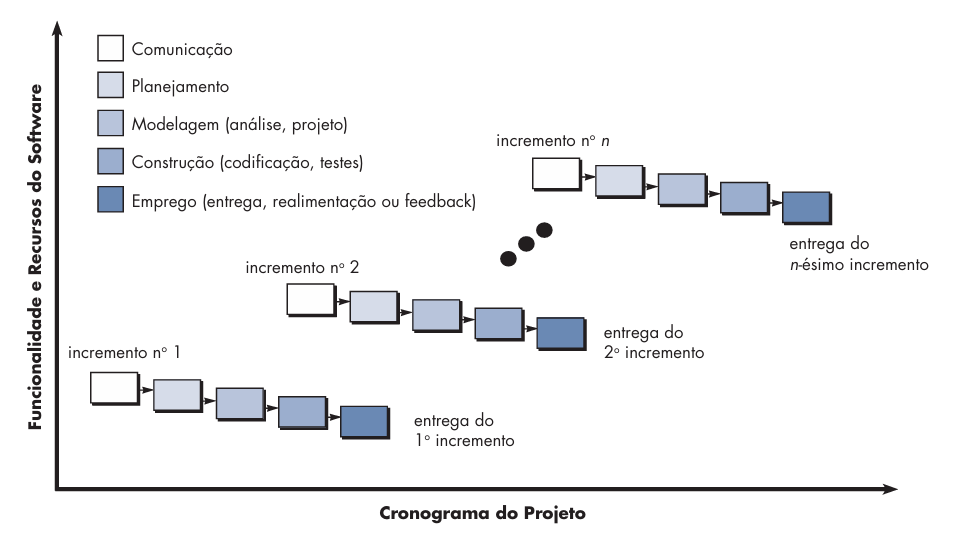
\includegraphics[width=0.8\textwidth]{imagens/graficoPressman.png}
  \caption{Ciclo de desenvolvimento incremental.}
  \legend{Fonte: \citeonline{pressman2011engenharia}.}
  \label{fig:incremental}
\end{figure}

% ---
\section{Kanban}
% ---

O Kanban é um método de gestão de fluxo de trabalho que fornece uma visualização das tarefas que devem ser realizadas, quando entregá-las e quanto ainda é necessário para finalizá-las com o objetivo de aumentar a eficiência e o entendimento do desenvolvimento \cite{ohno1988toyota}. Originou-se no sistema da Toyota no Japão dos anos 1940 e foi adaptado para o desenvolvimento de \textit{software} e sistemas de TI por David J. Anderson em 2004. Para isso, o Kanban utiliza de um quadro dividido em colunas para representar os diferentes estágios do trabalho, onde os cartões que representam as tarefas se movem de uma coluna para outra, refletindo o progresso real \cite{zayat2020framework}.

% ---
\section{Jira}
% ---

O \textit{Jira} é um \textit{software} comercial de gerenciamento de projetos desenvolvido pela empresa Atlassian. Ele permite a criação, acompanhamento e gerência de tarefas e projetos a partir de uma interface personalizável que suporta diversas metodologias ágeis como Scrum e Kanban, facilitando a colaboração e comunicação durante o desenvolvimento.

A ferramenta pode ser usada para planejar \textit{sprints}, atribuir tarefas, acompanhar \textit{bugs}, gerar relatórios e analisar o desempenho da equipe. Ele possui integração com uma variedade de ferramentas de desenvolvimento e oferece funcionalidades para personalizar fluxos de trabalho, campos e painéis, tornando-o adaptável às necessidades específicas de cada projeto ou organização.
